% Data flow diagram
% Author: David Fokkema
\documentclass{article}
\usepackage{tikz}
\usetikzlibrary{shapes,arrows}
\usepackage{pdflscape}
\usepackage[papersize={8cm, 3.6cm}, text={8cm, 4.6cm}]{geometry}
\usetikzlibrary{decorations.text}
\usepackage{xcolor}
% \selectcolormodel{gray}

\begin{document}
\thispagestyle{empty}
%\begin{landscape}
\begin{center}
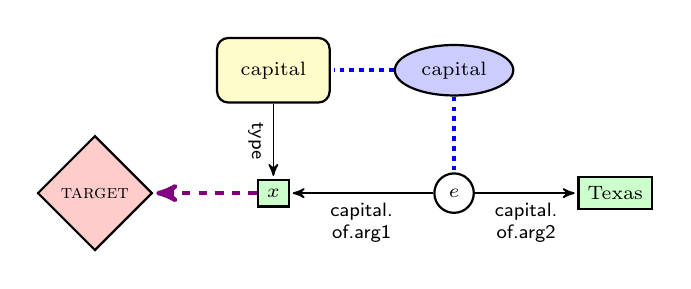
\begin{tikzpicture}[
  font=\sffamily,
  every matrix/.style={ampersand replacement=\&,column sep=0.8cm,row
sep=0.4cm,font=\scriptsize},
  entity/.style={draw,thick,rectangle,fill=green!20,font=\scriptsize},
  word/.style={draw,thick,ellipse,fill=blue!20},
  mediator/.style={draw,thick,circle},
  entityType/.style={draw,thick,rounded corners,fill=yellow!20,inner
sep=.3cm,font=\scriptsize},
  mathType/.style={draw,thick,diamond,fill=red!20,font=\sc\scriptsize},
  mediatorToEntity/.style={->,>=stealth',shorten
>=1pt,semithick,black,sloped,above,font=\sffamily\scriptsize},
  typeToEntity/.style={->,>=stealth',shorten
>=1pt,semithick,black,sloped,above,font=\sffamily\scriptsize},
  wordToEntity/.style={-,>=stealth',shorten >=1pt,ultra
thick,dotted,blue,sloped,above,font=\sffamily\scriptsize},
  entityToMath/.style={->,>=stealth',shorten >=1pt,ultra
thick,dashed,violet,sloped,above,font=\sffamily\scriptsize},
  every node/.style={align=center}]

  % Austin is the capital of Texas 
  
  % Position the nodes using a matrix layout
  \matrix{ 
   \& \node[entityType] (tCapital) {capital}; \& \node[word]
(wCapital) {capital}; \\
  \node[mathType] (mTarget) {target};  \& \node[entity] (eAustin) {$x$}; \&
\node[mediator]
(mCapital)  {$e$}; \& \node[entity]
(eTexas) {Texas}; \\
  };
 
  % words to entities
  %\draw [wordToEntity] (wAustin) edge node {}  (eAustin);
  %\draw [wordToEntity] (wTexas) edge node {}  (eTexas);
  % words to types
  \draw [wordToEntity] (wCapital) edge node {}  (tCapital);
  
  % type to entity
  \draw [typeToEntity][below] (tCapital) edge node {type}  (eAustin);
  
  % event word to mediators
  \draw [wordToEntity] (wCapital) edge node {}  (mCapital);
  
  % mediator to entities
  \draw [mediatorToEntity][below] (mCapital) edge node {capital.\\of.arg1} 
(eAustin);
  \draw [mediatorToEntity][below] (mCapital) edge node {capital.\\of.arg2} 
(eTexas);
   
   \draw [entityToMath] (eAustin) edge node {}  (mTarget);
  
\end{tikzpicture} 
\scriptsize $\textsc{target}(x) \wedge \mbox{capital}(x) \wedge
\mbox{capital.of.arg1}(e, x) \wedge \mbox{capital.of.arg2}(e,
\mathrm{Texas})$
\end{center}
\end{document}